\section{Recursive Integrator Class}
\label{interface-integrator-recursive}

Evaluates integral over element, approximating the integrand by an interpolatory polymomials of two hierarchical orders (2 and 4 at the moment). The running integration error is approximated by the difference between the analytical integrals calculated from these two interpolatory polynomials. The higher order element is split into into sub-elements of lower order, and the integration proceeds recursively. Every time an element is split, its previous running error is subtracted from the total error, and the running errors of the sub-elements are added to the total error. Thus, the integration is terminated when total approximated error is below selected tolerance. Heap structure ordered by the approximate error of the element is used to avoid recursion. At every iteration the element with the worst error is selected and then refined. When splitting, the previously calculated points are not re-calculated but hierarchically re-used by sub-elements. The sub-element only needs to be refined to a higher hierarchical order, by adding more points. \\

\noindent
\textit{Possible improvement - Performance}. As the the refined element does not check if the neighboring elements are also being refined, so they both sample on the boundary twice. Does there exist a method to store/find intersection refinements faster than just compute 2nd time. Using order 4 for every new refined triangle we sample 9 new points, out of which 2 are being wasted, thus $22\%$ inefficient.

\begin{figure}[p]
    \centering
    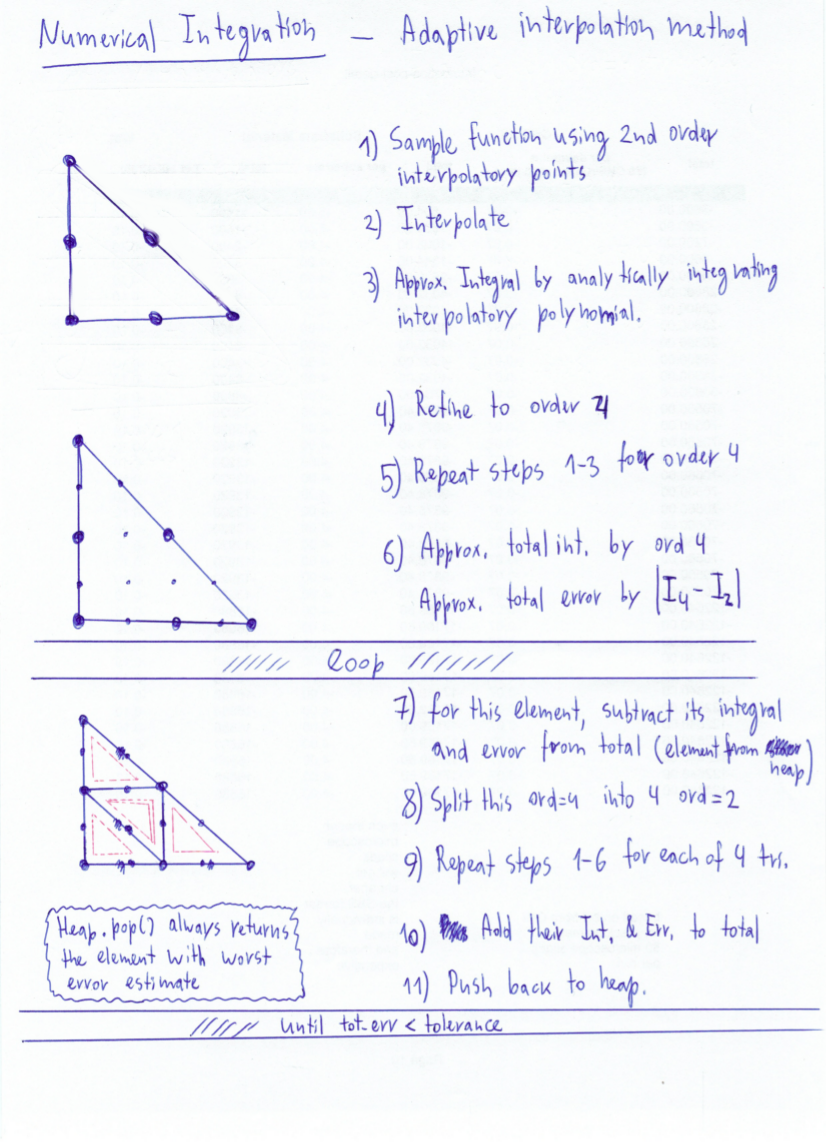
\includegraphics[scale=0.8]{doc-pics/pic-numerical-integration-adaptive-interpolation.png}
    %\caption{Awesome Image}
    %\label{fig:awesome_image}
\end{figure}


\subsection{Methods}
\label{interface-integrator-recursive-methods}

\noindent
Numerical Integration is only available for Simplices at the moment.

\noindent
\begin{itemize}
	\item \uline{Initialization:} Requires GeometryType to know the type of the element being integrated
	\item \uline{Integrate:} Integrates a function given by a functor object, until the expected integration error is below given tolerance.
\end{itemize}


\subsection{Tests}

\noindent
Numerical Integration is only implemented and hence tested for edges and triangles. A multitude of integrands are given in terms of Functors, starting with simple polynomial integrands and ending with integrands involving square roots of polynomials, as this is these are functions the method is expected to integrate well. The integrals are computed and compared to expected ones, which are sometimes given explicitly in numerical form, except of a lucky integral of $\iint \sqrt{xy} \; dxdy$ which happens to be $\pi / 24$. \\

\textbf{TODO:}
\begin{itemize}
	\item These tests should be automatized, which is easy to do, as they are only comparing numerical values.
	\item Integrals of complicated functions may exceed 100000 samples for this method given relative precision $10^{-5}$, which is too slow for the desired application
\end{itemize}